% Preámbulo
\documentclass[letterpaper]{article}
\usepackage[utf8]{inputenc}
\usepackage[spanish]{babel}

\usepackage{enumitem}
\usepackage{titling}

% Símbolos
	\usepackage{amsmath}
	\usepackage{amssymb}
	\usepackage{amsthm}
	\usepackage{amsfonts}
	\usepackage{mathtools}
	\usepackage{bbm}
	\usepackage[thinc]{esdiff}
	\allowdisplaybreaks

% Márgenes
	\usepackage
	[
		margin = 1.2in
	]
	{geometry}

% Imágenes
	\usepackage{float}
	\usepackage{graphicx}
	\graphicspath{{imagenes/}}
	\usepackage{subcaption}

% Ambientes
	\usepackage{amsthm}

	\theoremstyle{definition}
	\newtheorem{ejercicio}{Ejercicio}

	\newtheoremstyle{lemathm}{4pt}{0pt}{\itshape}{0pt}{\bfseries}{ --}{ }{\thmname{#1}\thmnumber{ #2}\thmnote{ (#3)}}
	\theoremstyle{lemathm}
	\newtheorem{lema}{Lema}

	\newtheoremstyle{lemathm}{4pt}{0pt}{\itshape}{0pt}{\bfseries}{ --}{ }{\thmname{#1}\thmnumber{ #2}\thmnote{ (#3)}}
	\theoremstyle{lemathm}
	\newtheorem{sol}{Solución}
	
	\newtheoremstyle{lemathm}{4pt}{0pt}{\itshape}{0pt}{\bfseries}{ --}{ }{\thmname{#1}\thmnumber{ #2}\thmnote{ (#3)}}
	\theoremstyle{lemathm}
	\newtheorem{theo}{Teorema}

	\newtheoremstyle{lemademthm}{0pt}{10pt}{\itshape}{ }{\mdseries}{ --}{ }{\thmname{#1}\thmnumber{ #2}\thmnote{ (#3)}}
	\theoremstyle{lemademthm}
	\newtheorem*{lemadem}{Demostración}

% Macros
	\newcommand{\sumi}[2]{\sum_{i=#1}^{#2}}
	\newcommand{\dint}[2]{\displaystyle\int_{#1}^{#2}}
	\newcommand{\inte}[2]{\int_{#1}^{#2}}
	\newcommand{\dlim}{\displaystyle\lim}
	\newcommand{\limtoinf}[1]{\lim_{#1\to\infty}}
	\newcommand{\dlimtoinf}[1]{\displaystyle\lim_{#1\to\infty}}
	\newcommand{\limtozero}[1]{\lim_{#1\to0}}
	\newcommand{\ddx}{\dfrac{d}{dx}}
	\newcommand{\txty}{\text{ y }}
	\newcommand{\txto}{\text{ o }}
	\newcommand{\Txty}{\quad\text{y}\quad}
	\newcommand{\Txto}{\quad\text{o}\quad}
	\newcommand{\si}{\text{si}\quad}

	\newcommand{\etiqueta}{\stepcounter{equation}\tag{\theequation}}
	\newcommand{\tq}{:}
	\renewcommand{\o}{\circ}
	\newcommand*{\QES}{\hfill\ensuremath{\blacksquare}}
	\newcommand*{\qes}{\hfill\ensuremath{\square}}
	\newcommand*{\QESHERE}{\tag*{$\blacksquare$}}
	\newcommand*{\qeshere}{\tag*{$\square$}}
	\newcommand*{\QED}{\hfill\ensuremath{\blacksquare}}
	\newcommand*{\QEDHERE}{\tag*{$\blacksquare$}}
	\newcommand*{\qel}{\hfill\ensuremath{\boxdot}}
	\newcommand*{\qelhere}{\tag*{$\boxdot$}}
	\renewcommand*{\qedhere}{\tag*{$\square$}}

	\newcommand{\suc}[1]{\left(#1_n\right)_{n\in\N}}
	\newcommand{\en}[2]{\binom{#1}{#2}}
	\newcommand{\upsum}[2]{U(#1,#2)}
	\newcommand{\lowsum}[2]{L(#1,#2)}
	\newcommand{\abs}[1]{\left| #1 \right| }
	\newcommand{\bars}[1]{\left \| #1 \right \| }
	\newcommand{\pars}[1]{\left( #1 \right) }
	\newcommand{\bracs}[1]{\left[ #1 \right] }
	\newcommand{\inprod}[1]{\left\langle #1 \right\rangle }
    \newcommand{\norm}[1]{\left\lVert#1\right\rVert}
    \newcommand{\floor}[1]{\left \lfloor #1 \right\rfloor }
	\newcommand{\ceil}[1]{\left \lceil #1 \right\rceil }
	\newcommand{\angles}[1]{\left \langle #1 \right\rangle }
	\newcommand{\set}[1]{\left \{ #1 \right\} }
	\newcommand{\norma}[2]{\left\| #1 \right\|_{#2} }


	\newcommand{\NN}{\mathbb{N}}
	\newcommand{\QQ}{\mathbb{Q}}
	\newcommand{\RR}{\mathbb{R}}
	\newcommand{\ZZ}{\mathbb{Z}}
	\newcommand{\PP}{\mathbb{P}}
    \newcommand{\EE}{\mathbb{E}}
	\newcommand{\1}{\mathbbm{1}}
	\newcommand{\eps}{\varepsilon}
	\newcommand{\ttF}{\mathtt{F}}
	\newcommand{\bfF}{\mathbf{F}}

	\newcommand{\To}{\longrightarrow}
	\newcommand{\mTo}{\longmapsto}
	\newcommand{\ssi}{\Longleftrightarrow}
	\newcommand{\sii}{\Leftrightarrow}
	\newcommand{\then}{\Rightarrow}

	\newcommand{\pTFC}{{\itshape 1er TFC\/}}
	\newcommand{\sTFC}{{\itshape 2do TFC\/}}


% Datos
    \title{Cálculo III \\ Tarea 1}
    \author{Rubén Pérez Palacios Lic. Computación Matemática\\Profesor: Fabián Augusto Pascual Domínguez}
    \date{\today}

% DOCUMENTO
\begin{document}
	\maketitle

	\begin{enumerate}
		\item Sea $\vec{x},\vec{y}\in \RR^n, n \geq 1$, entonces
		
		\begin{lema}
			Sea $V$ un espacio vectorial y $u,v \in V$ si $\norm{u} = \norm{v} = 1$ y $|\inprod{u,v}| = 1$ entonces $u$ y $v$ son linealmente dependientes.
		\end{lema}

		\begin{proof}
			Sean $u,v\in V$ entonces por linealidad del producto interior obtenemos

			\[\inprod{u\pm v,u\pm v} = \inprod{u,u}+\inprod{v,v} \pm 2\inprod{u,v},\]

			ahora si $\norm{u} = \norm{v} = 1$ entonces

			\[\inprod{u\pm v,u\pm v} = 2 \pm 2\inprod{u,v}.\]

			pero si $\inprod{u,v} = 1$ entonces

			\[\inprod{u-v,u-v} = 0,\]

			ahora puesto que $\inprod{x,x} = 0$ ssi $x=\vec{0}$ entonces

			\[u-v = \vec{0},\]

			por lo tanto concluimos que

			\[u = v.\]

			De manera análoga se obtiene para $\inprod{u,v} = -1$ considerando $\inprod{u+v,u+v}$.

		\end{proof}
		
		\begin{enumerate}
			\item $\abs{\vec{x}\cdot\vec{y}} = \norm{\vec{x}}\norm{\vec{y}}$ si y sólo si $\vec{x}$ y $\vec{y}$ son linealmente dependientes.
			
			\begin{proof}
				Si $\vec{x}$ y $\vec{y}$ son linealmente dependientes, entonces existe un $\lambda\in\RR$ tal que $\lambda x = y$, por lo que

				\begin{align*}
					\abs{\vec{x}\cdot\vec{y}} &= \abs{\vec{x}\cdot\lambda\vec{x}} &\text{Por ser linealmente dependientes $\vec{x}$ y $\vec{y}$}\\
					&= \abs{\lambda}\abs{\vec{x}\cdot\vec{x}} &\text{Por linealidad del producto punto}\\
					& &\text{y homogeneidad del valor absoluto}\\
					&= \abs{\lambda}\norm{x}\norm{x} &\text{Por relación producto punto y norma}\\
					&= \norm{x}\norm{\lambda x} &\text{Por homogeneidad de la norma}\\
					&= \norm{x}\norm{y}\\
				\end{align*}

				Ahora si $\abs{\vec{x}\cdot\vec{y}} = \norm{\vec{x}}\norm{\vec{y}}$ entonces por linealidad del producto punto obtenemos

				\[\abs{\frac{\vec{x}}{\norm{x}}\cdot\frac{\vec{y}}{\norm{y}}} = 1.\]

				por el lema 1 tenemos

				\[\frac{\vec{x}}{\norm{x}} = \frac{\vec{y}}{\norm{y}}.\]

				por lo tanto concluimos

				\[\vec{x} = \frac{\norm{x}}{\norm{y}} \vec{y},\]

				es decir $x$ y $y$ son linealmente dependientes.
			\end{proof}
			\item $\norm{\vec{x}+\vec{y}} = \norm{\vec{x}}+\norm{\vec{y}}$ si y sólo si $\vec{x}$ y $\vec{y}$ son linealmente dependientes.
			
			\begin{proof}
				Si $\vec{x}$ y $\vec{y}$ son linealmente dependientes entonces existe $\lambda\in\RR$ talque $\lambda x = y$ luego por homogeneidad de la norma tenemos que

				\[\norm{\vec{x}+\vec{y}} = \norm{\vec{x}+\vec{\lambda x}} = \pars{\abs{\lambda}+1}\norm{\vec{x}} = \norm{\vec{x}} + \norm{\vec{y}}.\]

				Ahora veamos la suficiencia, empecemos por ver que

				\[\norm{\vec{x} + \vec{y}} = \norm{\vec{x}} + \norm{\vec{y}}\]

				si y solamente si (por ser la norma no negativa)

				\[\norm{\vec{x} + \vec{y}}^2 = \norm{\vec{x}}^2 + \norm{\vec{y}}^2 + 2\norm{\vec{x}}\norm{\vec{y}},\]
				
				por otra parte por la relación que hay entre el producto punto y la norma, y linealidad del producto punto obtenemos

				\[\norm{\vec{x}}^2 + \norm{\vec{y}}^2 + 2(x\cdot y) = \norm{\vec{x}}^2 + \norm{\vec{y}}^2 + 2\norm{\vec{x}}\norm{\vec{y}},\]

				es decir

				\[\frac{\vec{x}}{\norm{\vec{x}}}\cdot \frac{\vec{y}}{\norm{\vec{y}}} = 1\]

				por el lema 1 obtenemos

				\[\vec{x} = \frac{\norm{\vec{x}}}{\norm{\vec{y}}} \vec{y},\]

				por lo tanto concluimos que $x$ y $y$ son linealmente dependientes.
			\end{proof}
			
		\end{enumerate}

		\item Sea $x\in\RR^n$ se cumple que
		
		\[\limtoinf{p} \norm{\vec{x}}_p = \norm{\vec{x}}_{\infty}.\]

		\begin{proof}
			Denotemos a $\sup\set{x_1,\cdots,x_n} = \sup\pars{x}$ el cual existe por se un conjunto finito, luego veamos que

			\[\norm{\vec{x}}_p = \pars{\sum_{i=1}^n |x_i|^{p}}^{\frac{1}{p}} \leq \pars{\sum_{i=1}^n \sup\pars{x}^{p}}^{\frac{1}{p}} = n^{\frac{1}{p}}\sup\pars{x}.\]

			Ahora

			\[\norm{\vec{x}}_p = \pars{\sum_{i=1}^n |x_i|^{p}}^{\frac{1}{p}} \geq \pars{\sup\pars{x}^{p}}^{\frac{1}{p}} = \sup\pars{x} \sup\pars{x} = \norm{x}_{\infty},\]

			por lo que

			\[\sup\pars{x} \leq \norm{\vec{x}}_p \leq n^{\frac{1}{p}}\sup\pars{x}.\]

			Recordemos que $\limtoinf{p} \frac{1}{p} = 0$, luego como $n^p$ es una función continua con $p\in\RR$ entonces $\limtoinf{p}n^{\frac{1}{p}} = 1$. Retomando la desigualdad anterior, junto con que los límites preservan el orden obtenemos

			\[\sup\pars{x} \leq \limtoinf{p} \norm{\vec{x}}_p \leq \sup\pars{x},\]

			es decir

			\[\norm{\vec{x}}_{\infty} \leq \limtoinf{p} \norm{\vec{x}}_p \leq \norm{\vec{x}}_{\infty},\]

			por lo tanto concluimos

			\[\limtoinf{p}\norm{\vec{x}}_p = \norm{\vec{x}}_{\infty}.\]
		\end{proof}

		\item Sean $\vec{x},\vec{y}\in\RR^n$
		
		\begin{enumerate}
			\item Mostrar que $\norm{x+y}^2 + \norm{x-y}^2 = 2\pars{\norm{x}^2+\norm{y}^2}$ (Ley del paralelogramo) e interpretar geométricamente.
			
			\begin{proof}
				Empecemos por ver que

				\[\norm{x\pm y}^2 = \pars{x\pm y}\cdot\pars{x\pm y} = \norm{x}^2 + \norm{y}^2 \pm 2\norm{x}\norm{y},\]

				por lo que concluimos que 

				\[\norm{x+y}^2 + \norm{x-y}^2 = 2\pars{\norm{x}^2+\norm{y}^2}.\]
			\end{proof}

			Geométricamente esto quiere decir que la suma del cuadrado de las  magnitudes de las diagonales de un paralelogramo es igual a la suma del cuadrado de los lados de este.

			\begin{figure}[H]
				\begin{center}
					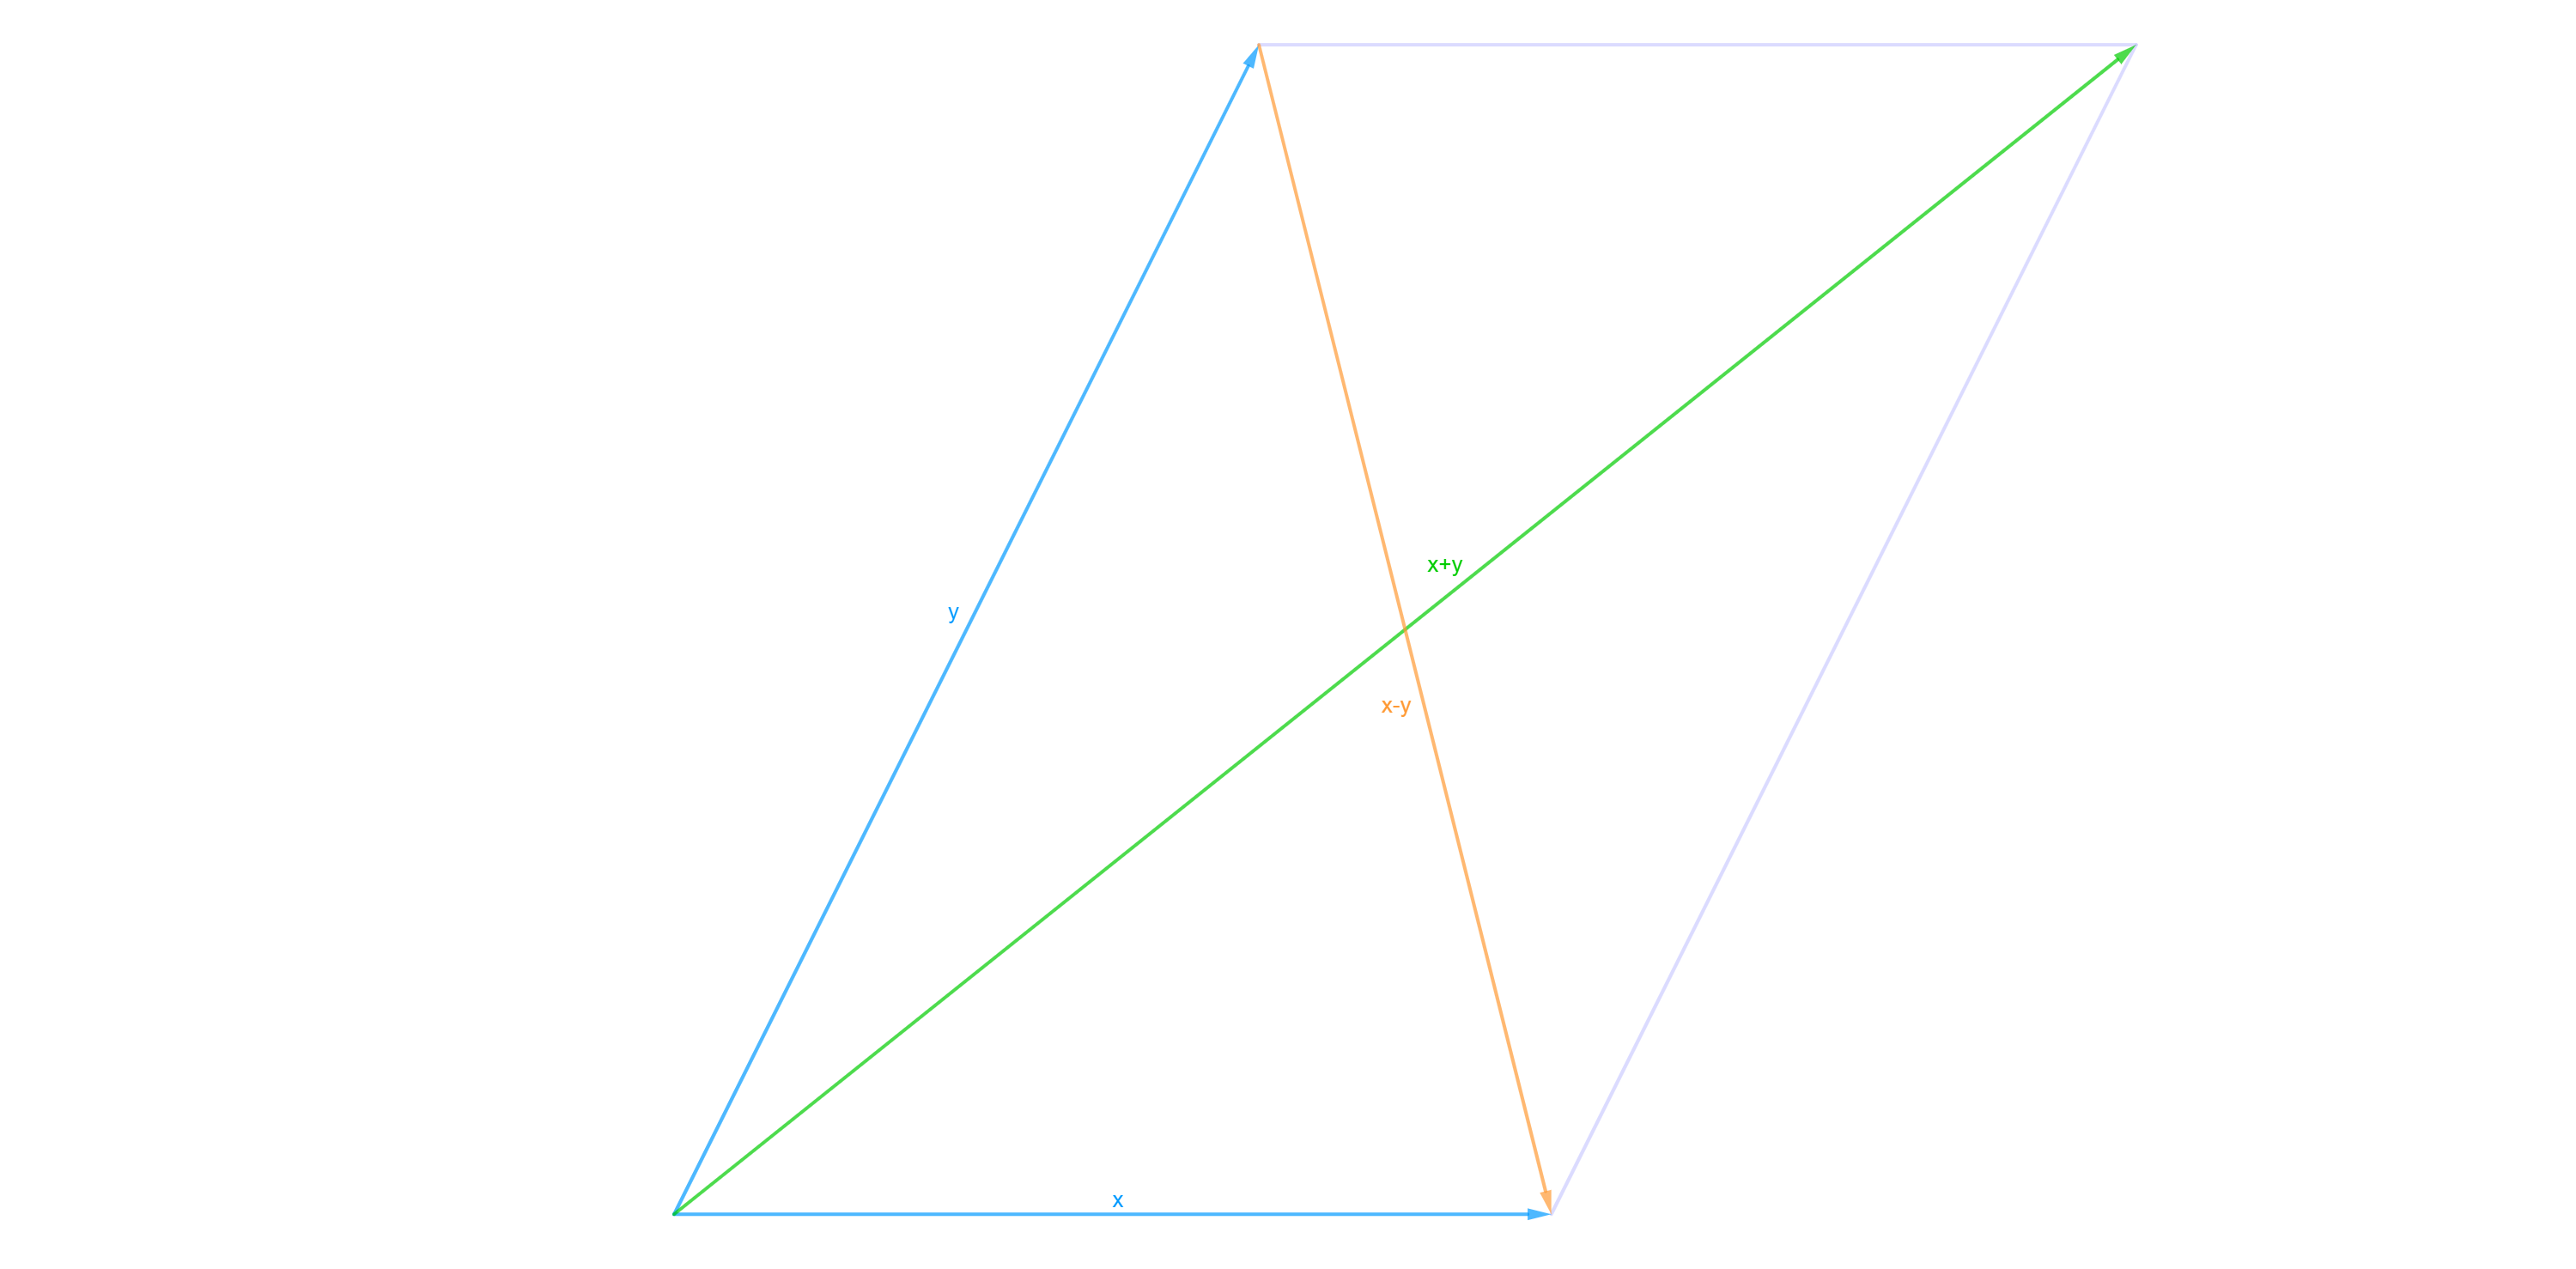
\includegraphics[scale = 1]{Images/Parallelogram.png}
				\end{center}
			\end{figure}

			Nota: En $\RR$ tenemos que $\norm{x}_{1} = \norm{x}_{\infty} = \norm{x} = \abs{x}$ por lo que en $\RR$ también es valida la ley del paralelogramo para estas normas.

			\item Probar que $\norm{\cdot}_{1}:\RR^n\rightarrow\RR, n \geq 2$ no satisface la ley del paralelogramo
			
			\begin{proof}
				Para $\vec{x} = \pars{1,0,\cdots,0}$ y $\vec{y} = \pars{0,\cdots,0,1}$ tenemos que

				\[\norm{x+y}_{1}^2 + \norm{x-y}_{1}^2 = 4n^2+4n^2 = 8n^2.\]

				pero

				\[2\pars{\norm{x}_{1}^2 + \norm{y}_{1}^2} = 2\pars{n^2+n^2} = 4n^2,\]

				por lo tanto la ley del paralelogramo no se cumple con $\norm{\cdot}_{1}$.
			\end{proof}

			\item Probar que $\norm{\cdot}_{\infty}:\RR^n\rightarrow\RR, n \geq 2$ no satisface la ley del paralelogramo
			
			\begin{proof}
				Para $\vec{x} = \pars{1,0,\cdots,0}$ y $\vec{y} = \pars{0,\cdots,0,1}$ tenemos que

				\[\norm{x+y}_{1}^2 + \norm{x-y}_{1}^2 = n^2+n^2 = 2n^2.\]

				pero

				\[2\pars{\norm{x}_{1}^2 + \norm{y}_{1}^2} = 2\pars{n^2+n^2} = 4n^2,\]

				por lo tanto la ley del paralelogramo no se cumple con $\norm{\cdot}_{\infty}$.
			\end{proof}

			\item Probar que $\norm{\vec{x}+\vec{y}}\norm{\vec{x}-\vec{y}}\leq\norm{\vec{x}}^2+\norm{\vec{y}}^2$.
			\begin{proof}
				Por MA-MG, la relación entre producto punto y norma, y linealidad del producto punto concluimos

				\[\norm{\vec{x}+\vec{y}}\norm{\vec{x}-\vec{y}} \leq \frac{\norm{\vec{x}+\vec{y}}^2 + \norm{\vec{x}-\vec{y}}^2}{2} = \frac{\inprod{\vec{x}+\vec{y},\vec{x}+\vec{y}} + \inprod{\vec{x}-\vec{y},\vec{x}-\vec{y}}}{2} =  \norm{\vec{x}}^2+\norm{\vec{y}}^2.\]
			\end{proof}
		\end{enumerate}

		\newpage

		\item ¿Son o no correctas las siguientes desigualdades, para todo $\vec{x},\vec{y}\in\RR^n$?
		
		\begin{enumerate}
			\item $\abs{\vec{x}\cdot\vec{y}} \leq \norm{\vec{x}}_{1}\norm{\vec{y}}_{1}$
			
			Primero veamos que

			\[\norm{\vec{x}}^2 = \sum_{i=1}^n \abs{x_i}^2 \leq \sum_{i=1}^n \abs{x_i}^2 + 2\sum_{i,j,i\neq j}\abs{x_i}\abs{x_j} = \norm{\vec{x}}_{1}^2,\]

			por lo 	que $\norm{\vec{x}} \leq \norm{\vec{x}}_{1}$. Por la desigualdad de Cauchy Schwarz y lo anterior concluimos que
			
			\[\abs{\vec{x}\cdot\vec{y}} \leq \norm{\vec{x}}_{1}\norm{\vec{y}}_1.\]

			\item $\abs{\vec{x}\cdot\vec{y}} \leq \norm{\vec{x}}_{\infty}\norm{\vec{y}}_{\infty}$
			
			Esto no es cierto puesto que para los vectores $\vec{x} = \pars{1,\cdots,1},\vec{y}=\pars{1,\cdots,1}$ tenemos que $\norm{\vec{x}}_{\infty} = \norm{\vec{y}}_{\infty} = 1$ y $\abs{\vec{x}\cdot\vec{y}} = n$ y entonces

			\[\abs{\vec{x}\cdot\vec{y}} = n \geq 1 = \norm{\vec{x}}_{\infty} \norm{\vec{y}}_{\infty}\]
		\end{enumerate}

		\item Sea $T:\RR^n\to\RR^m$ una aplicación lineal. Demostrar que existe un número $M$ positivo tal que
		
		\[\norm{T\pars{\vec{x}}} \leq M \norm{\vec{x}}, \forall x\in\RR^n.\]

		\begin{proof}
			Sea $\set{e_1,\cdots,e_n}$ la base canónica de $R^n$ luego

			\[\vec{x} = \sum_{i=1}^n x_i\vec{e}_i,\]

			por definición de norma obtenemos

			\[\norm{T\pars{\vec{x}}} = \norm{T\pars{\sum_{i=1}^n x_i\vec{e}_i}} = \norm{\sum_{i=1}^n x_i T\pars{\vec{e}_i}} \leq \sum_{i=1}^n \abs{x_i}\norm{T\pars{\vec{e}_i}}.\]

			luego tomemos $C_1 = \sup_i\set{T\pars{\vec{e}_i}}$ el cual existe por ser un conjunto finito en un campo completo, por úlitmo por la desigualdad de Cauchy Schwarz tenemos que si $\vec{\abs{x}} = \pars{\abs{x_1},\cdots,\abs{x_n}}$ donde $\vec{x} = \pars{x_1,\cdots,x_n}$ entonces
			
			\[\sqrt{n} \norm{\vec{x}} = \norm{\vec{\pars{1,\cdots,1}}} \norm{\vec{\abs{x}}} \geq \vec{\pars{1,\cdots,1}}\cdot\vec{\abs{x}} = \norm{\vec{x}}_1.\]

			Tomando a $M = C_1\sqrt{n}$ concluimos que

			\[\norm{T\pars{\vec{x}}} \leq M\norm{\vec{x}}\]
		\end{proof}

		\item Sea $\rho:\RR^n\times\RR^n\to\RR$ dada por
		
		\[\rho\pars{\vec{x},\vec{y}} = \begin{cases}
			1 & x \neq y\\
			0 & x = y
		\end{cases},\]

		¿Es $\rho$ una métrica sobre $\RR^n$?

		\begin{proof}
			Comprobaremos que se cumplen los axiomas de una metrica para $\rho$:

			\begin{enumerate}
				\item Por definición tenemos que $\rho\pars{\vec{x},\vec{y}} = 0$ ssi $x=y$.
				\item Por definición tenemos que $\rho\pars{\vec{x},\vec{y}} = \rho\pars{\vec{y},\vec{x}}$.
				\item Primero notemos que $\rho\pars{\vec{x},\vec{y}} \leq 1$ para todo $\vec{x},\vec{y}\in\RR^n$ luego si al menos dos vectores de $\vec{x},\vec{y},\vec{z}$ son distintos entonces $\rho\pars{\vec{x},\vec{z}} + \rho\pars{\vec{z},\vec{y}} \geq 1$ y por lo tanto $\rho\pars{\vec{x},\vec{y}} \leq \rho\pars{\vec{x},\vec{z}} + \rho\pars{\vec{z},\vec{y}}$, si todo son iguales entonces $\rho\pars{\vec{x},\vec{y}} = 0 = 0 + 0 = \rho\pars{\vec{x},\vec{z}} + \rho\pars{\vec{z},\vec{y}}$, por lo tanto se cumple el 3er axioma.
			\end{enumerate}

			Concluimos que $\rho$ es métrica.
			
		\end{proof}

		Todo conjunto $A$ es abierto puesto que para todo punto $a\in A$ es punto interior de este ya que tenemos que para todo $0<r<1$ la $B_r(a) = {a}\subset A$.

		\item Sea $X \in R^n$ convexo y sean $\lambda_1,\cdots,\lambda_p \geq 0$ tales que $\sum_{i=1}^p \lambda_i = 1$. Si $x_1,\cdots,x_p \in X$ entonces
		
		\[\sum_{i=1}^p \lambda_ix_i \in X.\]

		A esta expresión se le llama combinación convexa.

		\begin{proof}
			Procederemos a demostrar por inducción

			\begin{itemize}
				\item \textbf{Casos base} p = 1, $x\in X$ entonces $x\in X$. p = 2, por definción se cumple.
				\item \textbf{Hipótesis de Inducción}
				Sean $\lambda_1,\cdots,\lambda_p \geq 0$ tales que $\sum_{i=1}^p \lambda_i = 1$ y $x_1,\cdots,x_p \in X$ entonces
		
				\[\sum_{i=1}^p \lambda_ix_i \in X, \forall p < n\]
				\item \textbf{Paso de Inducción}
				
				Si algún $\lambda_i = 0$ entonces nuestra combinación convexa sería de menos puntos que $n$ y por hipótesis de inducción esta estaría contenida en $X$. Ahora si $\lambda_i \neq 0$ para toda $i$ entonces $\lambda_i < 1$ para toda $i$ y por lo tanto $1 - \lambda_1 > 0$. Puesto que $\lambda_2+\cdots+\lambda_n = 1 - \lambda_1$ tenemos quen por hipotesis de inducción

				\[\sum_{i=2}^n \frac{\lambda_i}{1-\lambda_1}x_i \in X,\]

				por último, de nuevo por hipotesis de inducción concluimos que

				\[\sum_{i=1}^n \lambda_ix_i = \lambda_1x_1 + \pars{1-\lambda_1}\sum_{i=2}^n \frac{\lambda_i}{1-\lambda_1}x_i \in X.\]
			\end{itemize}

			Por Inducción Matemática concluimos que toda combinación convexa de un conjunto convexo pertenece a este.
		\end{proof}

		\newpage

		\item Probar que para todo $\vec{x},\vec{y}\in\RR^n$:
		
		\begin{enumerate}
			\item $\abs{\norm{\vec{x}}-\norm{\vec{y}}}\leq\norm{\vec{x}\pm\vec{y}}$
			
			\begin{proof}
				Empecemos por ver que por subatividad de la norma se cumple que

				\[\norm{\vec{x}} = \norm{\pars{\vec{x}\pm\vec{y}} \mp \vec{y}} \leq \norm{\vec{x} \pm \vec{y}} + \norm{\vec{y}},\]

				por lo que

				\[\norm{\vec{x}} - \norm{\vec{y}} \leq \norm{\vec{x}\pm\vec{y}},\]

				y también

				\[\norm{\vec{y}} - \norm{\vec{x}} \leq \norm{\vec{y}\pm\vec{x}} = \norm{\vec{x}\pm\vec{y}},\]

				por lo tanto concluimos

				\[\abs{\norm{\vec{x}}-\norm{\vec{y}}}\leq\norm{\vec{x}\pm\vec{y}}\]


			\end{proof}

		\end{enumerate}

	\end{enumerate}

	Nota: Para efectos de esta tarea se uso que el producto interior como el producto punto.
\end{document}

